\documentclass[11pt,a4paper]{article}
\usepackage[margin=2.4cm]{geometry}
\usepackage{graphicx}
\usepackage{booktabs}
\usepackage{amsmath}
\usepackage{caption}
\usepackage[hidelinks]{hyperref}
\usepackage{microtype}

\captionsetup{font=small,labelfont=bf}
\setlength{\parskip}{0.35em}

\title{\bfseries Boundary severance in road networks:\\
a geometric permutation test, with the Berlin Wall\\ and the Cyprus buffer zone}
\author{Leo Y. Zhang}
\date{30 August 2026}

\begin{document}
\maketitle

\begin{abstract}
\noindent
Political boundaries bend road networks, and the standard measure of that
bending is circuity: network distance divided by straight-line distance. The
difficulty is that boundaries are usually drawn along rivers, canals and
railways, which bend a network by themselves, so excess circuity across a
boundary may belong to the terrain rather than to the politics. We introduce a
severance ratio equipped with a \emph{geometric permutation null}: the same
boundary curve is rigidly re-placed within the same city, preserving its shape,
length and enclosed area while destroying its historical position, and the true
placement is scored against that empirical null. Two boundaries are measured.
At the United Nations Buffer Zone in Nicosia, still closed today, crossing costs
49.9\,\% additional network distance
(0/20 displaced placebos exceed it, $z = +12.35$).
At the former inner Berlin Wall, removed in 1989, crossing still costs
1.0\,\%, and in every one of four barrier specifications not one of
23 rotated placebos reaches the true placement; at a finer spacing
none of 71 placements does either ($p = 0.0139$). The effect is small
but persistent: it holds across 7 sampling specifications
(1.0097 to 1.0242, every cluster interval excluding 1), and it
\emph{strengthens} rather than weakens when trips crossing water and rail are
removed, rising to 1.0401. Correcting for physical barriers therefore
sharpens the boundary's own signature instead of explaining it away, because
the same-side control trips cross water almost as often
(71.2\,\%) as the boundary-crossing trips
(90.7\,\%). Thirty-seven years after removal, a faint but measurable
trace of the Wall survives in Berlin's road network --- roughly one part in
51 of the cost of a boundary that is still shut. The method, its validation suite and
the full pipeline are released as open source.
\end{abstract}

\section{Introduction}

That infrastructure carries politics is an old claim and a well-evidenced one.
Haussmann's boulevards were cut partly to defeat barricades; the Russian
1520\,mm rail gauge differs from the European 1435\,mm standard; the interstate
programme in the United States was driven through Black neighbourhoods in
St.\ Paul, Detroit and New Orleans. The claim also has a famous cautionary tale.
Winner \cite{winner1980} reported that Robert Moses built the Long Island
parkway bridges low so buses could not pass, excluding those without cars;
Joerges \cite{joerges1999} showed the story does not survive contact with the
evidence. The lesson is not that infrastructure lacks politics. It is that
inferring political intent from physical form is easy to do badly.

The quantitative literature has largely sidestepped intent and measured
geometry. Circuity --- network distance divided by great-circle distance, also
called the detour index or route factor --- is a standard network measure
\cite{giacomin2015,levinson2020}, with typical motorway values near
$1.3 \pm 0.1$ \cite{npj2024}. Applied to borders, the OECD finds two cities in
the same country are roughly 10\,\% closer by road than two cities the same
distance apart across a national border \cite{oecd2013}, and cross-border
accessibility deficits in the European Union are well documented \cite{eu2019}.
A parallel public-health literature measures ``community severance'', the
barrier effect of roads on the neighbourhoods they cut \cite{severance2024}.
Separately, economists have used the division and reunification of Berlin as a
natural experiment on city structure, most prominently Ahlfeldt et al.\
\cite{ahlfeldt2015}, and Jedwab and Moradi have shown African colonial railway
cities persisted long after the railways stopped mattering \cite{jedwab2017}.

Two gaps sit between these literatures. The first is a missing reference point.
Excess circuity is normally assessed against $1$, or against a
whole-city average, but city geometry is not neutral: some parts of any city are
more circuitous than others for reasons that have nothing to do with any
boundary. The second is confounding. Boundaries follow rivers, ridges and rail
corridors precisely because those features are already hard to cross, so a study
that measures distortion across a political line risks attributing to politics
what belongs to hydrography --- and the error flatters the interesting
hypothesis.

\paragraph{Contributions.}
\begin{enumerate}\itemsep2pt
  \item A severance statistic for a boundary curve, defined on matched
    origin--destination pairs drawn from the same strip of city, so that
    crossing and non-crossing trips are compared like with like
    (Section~\ref{sec:stat}).
  \item A \emph{geometric permutation null}: rigid re-placement of the boundary
    curve within the same network, preserving shape, length and enclosed area,
    giving an exact empirical $p$-value with no distributional assumption
    (Section~\ref{sec:null}). We are not aware of this construction being used
    in this literature.
  \item A physical-barrier control implemented as a rasterised occupancy grid,
    giving constant-time segment--barrier queries, so water and rail crossings
    can be removed or held fixed (Section~\ref{sec:barriers}).
  \item A validation suite checking reconstructed geometry against independent
    ground truth before any result is computed (Section~\ref{sec:validation}),
    and an open, dependency-light implementation.
  \item Empirically: a large effect at a boundary still closed, a small but
    robust one at a boundary removed thirty-seven years ago, and the finding
    that barrier controls sharpen rather than explain the latter.
\end{enumerate}

\section{Data}

All data are from OpenStreetMap (OSM) via the Overpass API, retrieved
30 August 2026, and cached locally so runs are reproducible.

\paragraph{Road network.} We take ways tagged \texttt{highway} in the drivable
classes (motorway through living\_street, plus link roads), excluding areas and
ways tagged \texttt{access=no} or \texttt{private}. For Berlin this yields
106295 ways and 389092 nodes, from which we build an
undirected weighted graph with edge weights equal to the haversine length of
each consecutive node pair. Retaining the largest connected component leaves
386719 nodes and 406264 edges, or 99.4\,\%
of nodes. Nicosia yields 186900 nodes and 196808 edges;
Hamburg, used for a sensitivity check, yields 246572 nodes.

Treating the network as undirected is a simplification: it measures the
symmetric accessibility of two points rather than a specific driving manoeuvre.
It is the right choice here because the object of study is the shape of the
network, not turn-level routing.

\paragraph{The Wall.} The physical Wall survives only as fragments; OSM holds
just a handful of disconnected wall segments, too few to define a line. We
instead use the \emph{Berliner Mauerweg} (OSM relation 9030), the signposted
route maintained by the Berlin Senate that traces the former border strip. Its
1422 member ways include 71 tagged as
alternatives, plus forward/backward branch pairs, so naive endpoint chaining
shatters it into fragments. Chaining at an 11\,m snap tolerance and discarding
alternatives assembles a single closed loop of 5360 vertices and
158.2\,km closing to within 13.4\,m, against the relation's
declared 160\,km. The Mauerweg is a proxy: as a rideable path it deviates from
the exact border strip where that strip is now built over. We return to this in
Section~\ref{sec:limits}.

\paragraph{Inner and outer boundary.} The loop is not one boundary. Part of it
divided East from West Berlin; the rest separated West Berlin from surrounding
Brandenburg and still coincides with the Berlin state line. We separate them by
distance to Berlin's present administrative boundary
(6185 vertices), classifying ring vertices more than 400\,m
from the state line as inner. This gives 62.3\,km inner and
94.1\,km outer, against historical figures of approximately 43\,km and
112\,km; our inner segment is longer because the Mauerweg detours inside the
city limits in places. Only the inner segment is the East--West urban division,
and it is our object of study.

\paragraph{The buffer zone.} For Nicosia we use the disputed-boundary linestring
(OSM relation 13562321), whose longest chain gives 1419
vertices over 170.6\,km.

\paragraph{Barriers.} Water comes from ways tagged
\texttt{waterway=river\,|\,canal} and \texttt{natural=water}
(3063 polylines); rail from \texttt{railway=rail\,|\,light\_rail}
excluding tunnels (8212 polylines).

\section{Method}

\subsection{The severance statistic}\label{sec:stat}

Let $R$ be a closed boundary curve and $G=(V,E)$ the road graph. For an
origin--destination pair $(u,v)$ write $d_G(u,v)$ for the shortest-path distance
and $d_E(u,v)$ for the great-circle distance. Circuity is
\[
  c(u,v) \;=\; \frac{d_G(u,v)}{d_E(u,v)} \;\ge\; 1 .
\]
A pair is \textsc{cross} if exactly one endpoint lies inside $R$, and
\textsc{same} otherwise. The severance ratio is
\[
  S(R) \;=\; \frac{\operatorname{median}\,\{\,c(u,v) : (u,v)\in\textsc{cross}\,\}}
                  {\operatorname{median}\,\{\,c(u,v) : (u,v)\in\textsc{same}\,\}} .
\]
Medians are used because circuity has a heavy right tail. $S>1$ means crossing
the boundary costs extra detour beyond what trips of the same length in the same
place already pay.

The comparison is only meaningful if the two groups are otherwise alike, so both
are drawn under identical constraints: great-circle separation in
$[1, 6]$\,km, and pair midpoint within 1500\,m of the
boundary. The midpoint constraint is what makes the control group local ---
\textsc{same} pairs run alongside the boundary in the same neighbourhood rather
than anywhere in the city. Nodes within 150\,m of the line are dropped
as side-ambiguous, and at most 40 targets are kept per origin so no
origin dominates.

\subsection{The geometric permutation null}\label{sec:null}

The obvious test, $S>1$, is the wrong test, and our data show why: in Berlin the
placebo placements average $0.9827$, not $1$. Boundary-adjacent
strips of city are, on average, slightly \emph{less} circuitous to cross than to
travel along. Testing against $1$ would therefore be conservative in one
direction and misleading in the other.

We build the reference empirically instead. Let $T$ be a rigid transformation
--- a rotation about the curve's own centroid, or for an open boundary a
perpendicular displacement. $T(R)$ has the same shape, length and enclosed area
as $R$, and sits in the same city, but not where history put it. Computing
$S(T(R))$ over a family $\{T_i\}$ gives a null distribution, with empirical
$p$-value
\[
  p \;=\; \frac{1 + \#\{ i : S(T_i(R)) \ge S(R) \}}{1 + n} .
\]
For Berlin we use 23 rotations at $15^{\circ}$ intervals. Nicosia's
boundary is a line, for which rotation about a centroid is meaningless, so we
use perpendicular displacements of 2 to 12\,km either side
(20 placebos).

This is the central methodological move. It converts ``is there excess
circuity?'' --- which the geometry of any city will answer yes to somewhere ---
into ``is there more excess circuity here than at comparable placements of the
same curve?'', which is the question actually being asked.

\subsection{Physical-barrier control}\label{sec:barriers}

Boundaries follow rivers. To separate the two we rasterise water and rail
polylines onto a boolean occupancy grid at 20\,m resolution
(Berlin: 1.02\,\% of cells water, 0.79\,\%
rail). Testing whether a straight segment meets a barrier is then a walk along
the segment with constant-time lookups, rather than a comparison against every
barrier polyline. The first and last 60\,m of each segment are skipped so a road
running along a quayside is not counted as crossing the water beside it.

We apply this two ways. \emph{Removing} the confound drops every pair whose
straight line meets a barrier, isolating trips for which no physical obstacle
other than the boundary is present. \emph{Holding it constant} keeps only pairs
that all cross water, so both groups pay the water penalty and any remaining gap
cannot be hydrography.

\subsection{Implementation}

The pipeline is Python with only \texttt{numpy} and \texttt{scipy} beyond the
standard library; no geospatial stack is required. Shortest paths use SciPy's
Dijkstra over a CSR sparse matrix, run in batches of 40 origins with a distance
cut-off, keeping the working set bounded while amortising traversal. Proximity
queries --- distance from every node to the boundary, and from every pair
midpoint --- use a $k$-d tree over boundary vertices; with vertex spacing near
30\,m this approximates true point-to-polyline distance to within about 15\,m.
Point-in-polygon uses vectorised ray-casting parity evaluated over all candidate
nodes at once on a decimated ring. On a 16-core laptop one placement over the
386719-node Berlin graph with 600 origins takes under a
minute, so a full 24-placement experiment runs in about a quarter of an hour.

\subsection{Validation}\label{sec:validation}

Reconstructed geometry is checked against independent ground truth before any
result is computed; if a check fails the pipeline stops. The assembled Wall ring
encloses 473.3\,km$^2$ against West Berlin's actual 480\,km$^2$, an
error of 1.4\,\%. All 18 landmark tests pass:
8 West Berlin locations (Charlottenburg Palace, Tempelhofer Feld,
Spandau, Wedding and others) fall inside the ring and 10 East Berlin and
Brandenburg locations (Alexanderplatz, Karl-Marx-Allee, K\"openick, Teltow and
others) fall outside. For Cyprus all 7 landmark tests pass,
with north Nicosia, Kyrenia and G\"onyeli on one side and south Nicosia,
Strovolos, Lakatamia and Larnaca on the other. The Nicosia road network is a
single connected component across the buffer zone, so measured detours reflect
real routes through the crossing points rather than a severed graph.

\section{Results}

\begin{figure}[t]
\centering
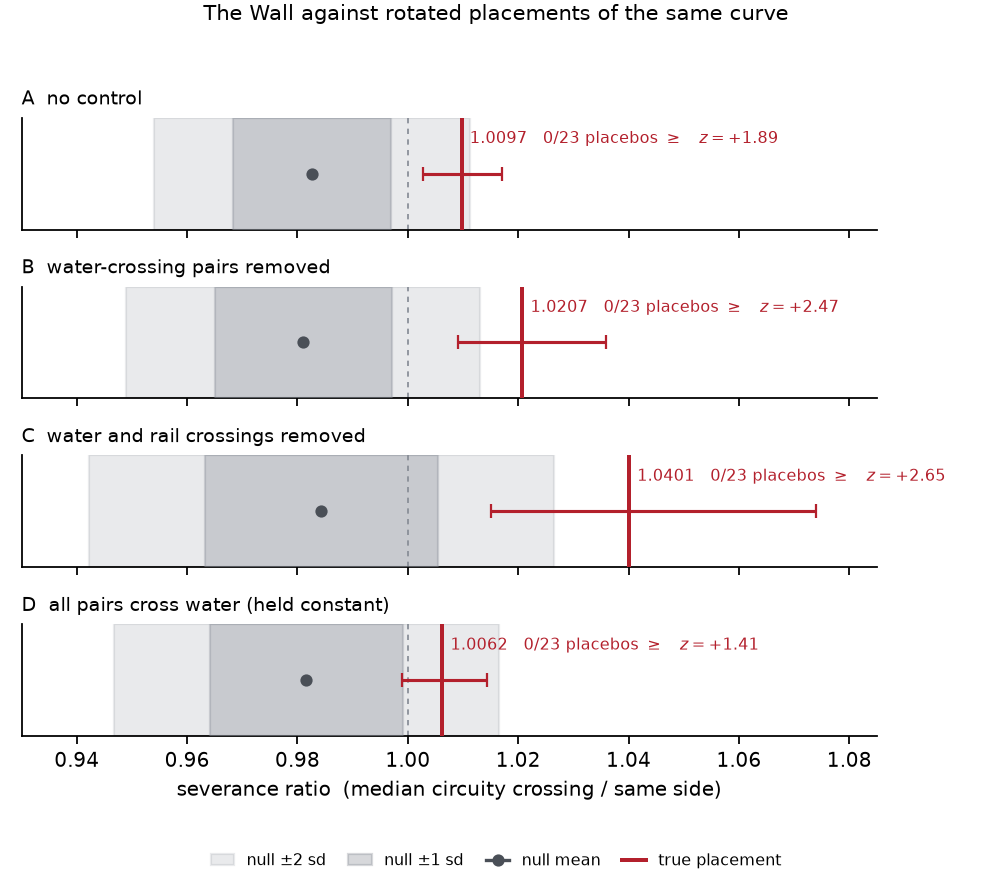
\includegraphics[width=0.98\linewidth]{fig2_nulls.png}
\caption{The Berlin measurement against its own null. Each grey point is the
severance ratio obtained when the identical boundary curve is rotated about its
centroid to a different placement in the same city; the red line is the true
historical placement. Panel A is the uncontrolled measurement; B and C remove
pairs crossing water, and water and rail; D keeps only pairs that all cross
water. The dashed line marks 1.0, which is \emph{not} the correct reference ---
the placebo clouds sit below it, which is why the null is built empirically.}
\label{fig:nulls}
\end{figure}

\subsection{Positive control: the buffer zone at Nicosia}

A result at a removed boundary is only interpretable if the method can detect a
present one, so we first measure a boundary still closed. Crossing the UN Buffer
Zone costs $S = 1.4991$, that is 49.9\,\% additional network distance
(cluster-bootstrap 95\,\% CI $[1.4276, 1.5733]$; $n = 11801$
crossing and $11152$ same-side pairs; $1.4840 \pm
0.0145$ across independent origin samples). The displaced placebos
average $1.0058$ with standard deviation $0.0399$;
0 of 20 reach the true value, giving $p = 0.048$ and
$z = +12.35$. The method detects a live boundary at eleven standard
deviations, and sets the scale against which Berlin should be read.

\subsection{The inner Berlin Wall}

\begin{table}[t]
\centering
\small
\begin{tabular}{lrccrr}
\toprule
Control & $S$ & 95\,\% CI (cluster) & placebo mean $\pm$ sd & placebos $\ge S$ & $z$ \\
\midrule
none                    & 1.0097 & $[1.0027,\ 1.0171]$ & 0.9827 $\pm$ 0.0143 & 0/23 & $+1.89$ \\
water removed           & 1.0207   & $[1.0092,\ 1.0360]$     & 0.9810 $\pm$ 0.0161     & 0/23   & $+2.47$ \\
water and rail removed  & 1.0401  & $[1.0150,\ 1.0740]$   & 0.9843 $\pm$ 0.0211   & 0/23  & $+2.65$ \\
water held constant     & 1.0062   & $[0.9990,\ 1.0143]$     & 0.9816 $\pm$ 0.0175     & 0/23   & $+1.41$ \\
\bottomrule
\end{tabular}
\caption{The Berlin effect under physical-barrier controls, each against its own
23-placement null, all at 600 origins so the rows are
comparable. In every specification no placebo reaches the true placement.}
\label{tab:controls}
\end{table}

Measured without controls, the former inner Wall gives $S = 1.0097$ ---
an excess of 1.0\,\% --- with 0 of 23 rotated
placebos reaching it ($p = 0.042$, $z = +1.89$). The effect is small. It
is also, on three separate checks, real.

\paragraph{Physical barriers sharpen it.} Our initial expectation was that the
effect would be an artefact of the Spree, since the Wall was routed along water
and rail for much of its length. Table~\ref{tab:controls} shows the opposite.
Removing pairs that cross water raises the estimate to 1.0207; removing
water and rail raises it to 1.0401, its largest value, at $z =
+2.65$. Restricting instead to pairs that \emph{all} cross water gives
1.0062, the smallest.

The explanation is that Berlin is a watery city and the confound cuts both ways.
Of 13377 pairs crossing the inner Wall, 90.7\,\%
also cross water and 86.1\,\% cross rail, with
99.0\,\% crossing one or the other --- but
71.2\,\% of the same-side control pairs cross water too.
Water is therefore not a rival explanation for the contrast between the groups;
it is noise common to both, and it \emph{dilutes} the boundary signal. Removing
it isolates trips whose only obstacle is the former boundary, and there the Wall
costs about 4.0\,\%. Where a river must be crossed anyway, the river
dominates and the Wall adds little.

\paragraph{A finer null.} With 23 placements the smallest
attainable $p$-value is $1/24$, which the headline
specification attained exactly --- the test could show the true placement was
extremal but not how extremal. Repeating it at 71 placements, one every
$5^{\circ}$, drops the floor to $1/72$. The result
(Figure~\ref{fig:finenull}) is unchanged in estimate and sharper in inference:
the null spans 0.9452 to 1.0070, and the highest of all 71
alternative placements, 1.0070, still falls below the true value of
1.0097. No rotation of the Wall's own shape, anywhere in Berlin, severs
the city as much as the position it actually occupied. This gives
$p = 0.0139$.

\paragraph{The estimate is stable.} Every threshold in Section~\ref{sec:stat} is
arbitrary within reason. Varying each singly (Table~\ref{tab:sens}) moves the
estimate only between 1.0097 and 1.0242, and every cluster interval
excludes 1.

\paragraph{Statistical dependence.} Pairs are not independent: up to
40 share an origin node and a single shortest-path tree, so a
bootstrap resampling \emph{pairs} reports a deceptively tight interval. On a
large run with 2000 origins ($S = 1.0122$, 42773 crossing pairs)
the naive interval is $[1.0107, 1.0139]$, whereas resampling
whole origin clusters widens it by a factor of 2.4 to
$[1.0085, 1.0163]$. All intervals reported here are the cluster
version. Repeating that run under 4 independent origin samples gives
$1.0129 \pm 0.0010$, so the estimate is stable once the sample
is adequate; at 150 origins it was not, swinging by more than the size of the
effect in both directions, which is a caution worth recording for anyone
reusing this design.

\begin{figure}[t]
\centering
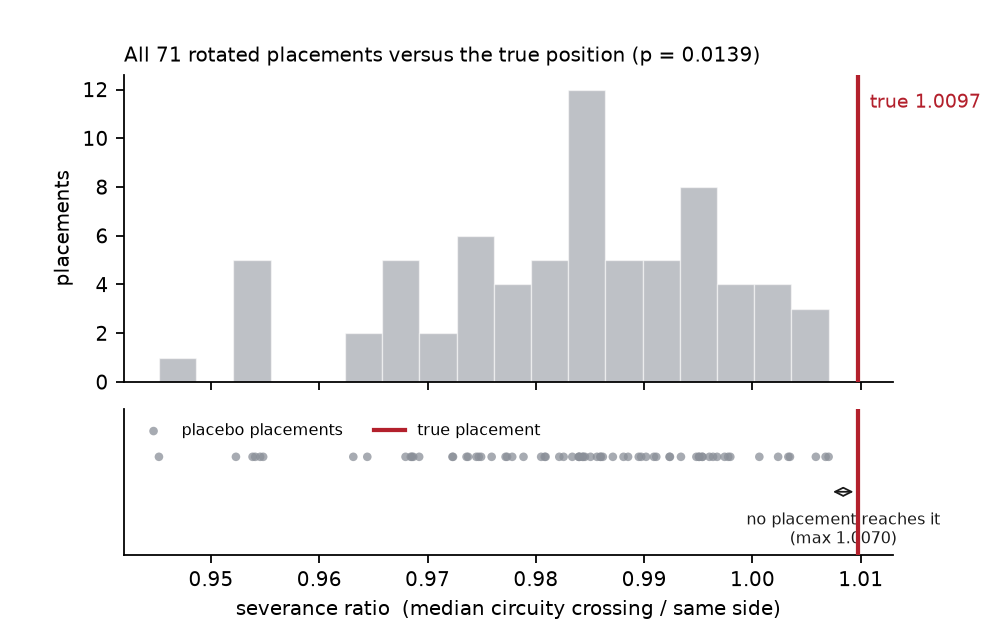
\includegraphics[width=0.94\linewidth]{fig3_finenull.png}
\caption{The headline specification against a finer null of 71 rotated
placements at $5^{\circ}$ intervals. Above, the distribution of placebo
severance ratios; below, the individual placements. The true position of the
Wall lies beyond every one of them.}
\label{fig:finenull}
\end{figure}

\begin{table}[t]
\centering
\small
\begin{tabular}{lrcr}
\toprule
Specification & $S$ & 95\,\% CI (cluster) & crossing pairs \\
\midrule
default & 1.0097 & $[1.0027,\ 1.0171]$ & 13377 \\
band 1000 m & 1.0210 & $[1.0139,\ 1.0268]$ & 15654 \\
band 2500 m & 1.0124 & $[1.0061,\ 1.0190]$ & 8227 \\
trips 0.5-3 km & 1.0242 & $[1.0166,\ 1.0327]$ & 5819 \\
trips 2-10 km & 1.0107 & $[1.0057,\ 1.0159]$ & 14435 \\
exclude 300 m & 1.0116 & $[1.0036,\ 1.0200]$ & 13000 \\
split tol 800 m & 1.0105 & $[1.0035,\ 1.0178]$ & 14006 \\
\bottomrule
\end{tabular}
\caption{Stability of the Berlin point estimate across sampling parameters, each
varied singly from the default, at 600 origins.}
\label{tab:sens}
\end{table}

\subsection{Where the residual sits}

\begin{figure}[t]
\centering
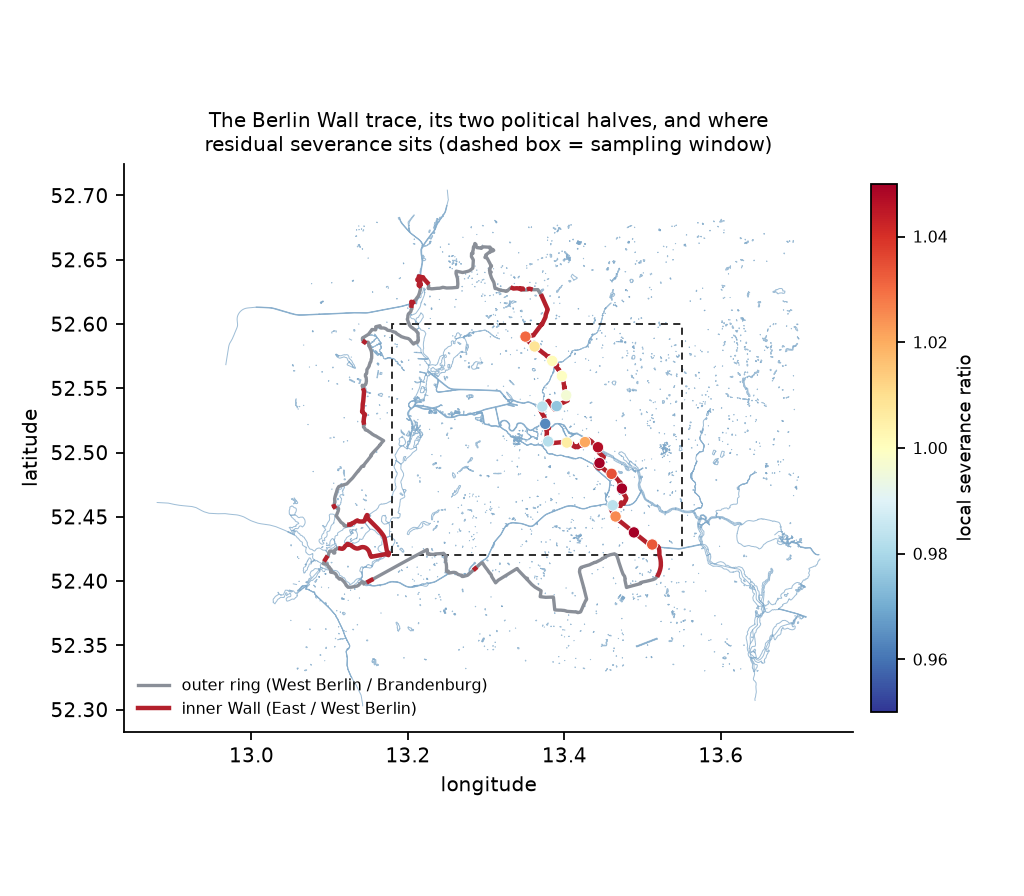
\includegraphics[width=0.92\linewidth]{fig1_map.png}
\caption{The reconstructed Wall trace over Berlin's water network, split into
the inner segment that divided East from West Berlin (red) and the outer segment
that separated West Berlin from Brandenburg (grey). Points show local severance
in 2\,km bins along the inner segment. The visible correlation between boundary
and water is what the barrier control in Table~\ref{tab:controls} addresses.}
\label{fig:map}
\end{figure}

Binning crossing pairs by position along the inner Wall (19 bins of
2\,km with at least 40 pairs each) shows the residual is not uniform:
12 of 19 bins exceed 1.0, with a median of
1.0088. The largest values lie in the south-east --- Plänterwald
1.161, Johannisthal-Süd 1.087, Kungerkiez 1.059 ---
while the smallest lie in the centre, at Friedrich-Wilhelm-Stadt 0.963 and
Oranienburger Vorstadt 0.975. The pattern is legible: the central districts
were the focus of post-1990 reconstruction, with Potsdamer Platz, the government
quarter and the new central station rebuilt across the former line, while the
south-eastern stretch through Treptow and Johannisthal received far less.

\subsection{The statistic responds to physical geography}

Transplanting the Berlin curve onto Hamburg, a comparable city never
partitioned, gives severance ratios from 0.8919 to 1.5082 across
24 placements, with 3 above 1.05. Hamburg's port and the Elbe
are enough to produce large apparent severance from an arbitrary curve. This is
not a defect --- a river genuinely does sever a road network --- but it shows
that a raw circuity excess, absent a null, carries little information about
politics. It is also why the null must be built inside the same city: a
comparison across cities compares harbours, not boundaries.

\section{Discussion}

\subsection{What Berlin shows}

Thirty-seven years after the Wall was removed, crossing its former line still
costs measurably more than travelling the same distance alongside it, and more
than the same curve costs anywhere else in Berlin. The effect is small ---
around 1.0\,\% in general traffic, around 4.0\,\% where no
river or railway intervenes --- and it should be read against the
49.9\,\% at Nicosia. A boundary still closed costs roughly a factor of
51 more than one taken down a generation ago. Berlin has very
largely, but not completely, healed.

We are careful about how far to push this. The measurement covers the drivable
network only. It says nothing about rail, cycling or walking, nothing about who
actually travels, and nothing about the economic and social asymmetries that
Ahlfeldt et al.\ \cite{ahlfeldt2015} document and that remain visible in rents,
firm location and demography. A city can be close to topologically healed and
still divided in every way that matters to the people in it. Our result is about
road geometry, and only that.

\subsection{On confounding, in both directions}

We began expecting to find that the Wall's apparent signature was really the
Spree. That expectation was wrong, and the way it was wrong is instructive.
Because the control group is drawn from the same strip of city, it inherits the
same rivers: 71.2\,\% of same-side pairs cross water against
90.7\,\% of crossing pairs. A confound shared by treatment and
control is not a rival explanation --- it is attenuation. Removing it does not
deflate the estimate; it deflates the noise.

This cuts against a natural instinct to treat every control as a threat to be
survived. The direction a control moves an estimate is itself evidence. Had the
barrier control reduced our effect towards the null, the collinearity story
would have been right; it raised it, which points the other way. We would argue
that reporting the direction of movement under controls, rather than only
whether significance survives, should be routine.

The wider caution still stands, and Hamburg demonstrates it: an arbitrary curve
laid across a port city yields ratios up to 1.5082 with no politics
whatever. Circuity excess without a null is not a finding. The permutation
construction is cheap --- 23 extra runs of the same code --- and we think it
should be standard in this literature.

\subsection{Limitations}\label{sec:limits}

\textbf{The Mauerweg is a proxy.} It follows the border strip but deviates onto
rideable ground where the original line is built over, which is why our inner
segment measures 62.3\,km against a historical 43\,km. Errors of tens of
metres are immaterial at our trip lengths; systematic detours are not, and a
study of the exact 1989 cadastral line might differ.

\textbf{The null is finite.} A permutation null of $n$ placements cannot report
a $p$-value below $1/(n+1)$. At 23 placements every Berlin
specification attained that floor exactly. Extending the headline specification
to 71 placements lowered the floor to 0.0139, which it again attained,
so the constraint has been relaxed rather than removed. The remaining three
specifications are still reported at 23 placements and remain
floored; their $z$ scores, which are not floored, carry the finer information.
Extending them is a matter of compute only.

\textbf{Rotations are not perfectly exchangeable.} A rotated ring samples
different parts of the city, and Berlin's built form is not isotropic. The
Hamburg transplant shows how much placement alone can matter.

\textbf{OSM completeness is uneven}, varying sharply with development level
\cite{osm2023}. Berlin, Hamburg and Nicosia are all well mapped, so this limits
generalisation rather than these results.

\textbf{Distance, not time.} We ignore one-way restrictions, turn costs and
speeds. Travel time would arguably be the better severance measure and needs
data we do not have.

\subsection{Further work}

The natural next step is comparative. The apparatus is boundary-agnostic --- it
needs a curve, a road network and a null --- so the same instrument could be run
across internal apartheid-era buffer strips, the ceasefire line in Kashmir and
motorway severance in postwar American cities, and asked whether severance sorts
by boundary type, by age, or by whether the boundary is still enforced. Our two
points hint at such a curve; a dozen would begin to define one.

The binding constraint is boundary geometry, not method. We attempted Belfast,
which would have been the informative middle case, since many peace lines still
stand and some have gates closed nightly. It could not be done: of roughly 1,300
ways tagged as walls within the Belfast bounding box, exactly one carries a tag
identifying it as a peace line. The barriers are physically present and
politically documented, but they are not distinguishable in the map data, so the
geometry would have to be digitised from the Northern Ireland barrier register
before this method could touch them. Anyone extending this work should budget
for boundary digitisation rather than assuming, as we initially did, that a
mapped wall is a findable wall. A second direction is temporal: OSM history would in
principle allow the Berlin measurement to be repeated for 2010 and 2020, turning
two endpoints into a healing trajectory.

\section{Conclusion}

We set out to test whether a removed political boundary still bends a city's
road network, and built an instrument with a geometric permutation null to do
it. At Nicosia, where the boundary is still closed, it registers 49.9\,\%
excess circuity at $z = +12.35$, with not one of 20 displaced
placebos coming close. At Berlin it registers 1.0\,\% --- small, but
present in every specification we tried, stable across sampling parameters, and
never once matched by any of 23 alternative placements of the same
curve.

The methodological lesson is the one we did not expect. We built the barrier
control believing it would explain the Berlin effect away, and it did the
reverse: because the control trips cross the same rivers, the water was
attenuating the signal rather than creating it. Confounds shared between
treatment and control do not inflate an effect, they hide it --- and the
direction a control moves an estimate is worth reporting whether or not
significance survives.

\section*{Reproducibility}

The full pipeline --- data retrieval, geometry assembly, validation, measurement
and every figure and number in this paper --- is available as open source,
depending only on \texttt{numpy} and \texttt{scipy} beyond the Python standard
library. Overpass responses are cached, and the manuscript's numerical values
are injected programmatically from the result files rather than transcribed,
with the build failing if any value is missing, so the text cannot drift from
the analysis.

\begin{thebibliography}{99}\small
\bibitem{winner1980} L.~Winner. Do artifacts have politics? \emph{Daedalus}
  109(1):121--136, 1980.
\bibitem{joerges1999} B.~Joerges. Do politics have artefacts?
  \emph{Social Studies of Science} 29(3):411--431, 1999.
\bibitem{giacomin2015} D.~J.~Giacomin and D.~M.~Levinson. Road network circuity
  in metropolitan areas. \emph{Environment and Planning B} 42(6):1040--1053, 2015.
\bibitem{levinson2020} S.~Sarkar, D.~Wu and D.~M.~Levinson. Measuring
  polycentricity via network circuity. \emph{Spatial Information Research}, 2020.
\bibitem{npj2024} How much longer do you have to drive than the crow has to fly?
  \emph{npj Complexity} 1, 2024.
\bibitem{oecd2013} Road connectivity and the border effect. OECD, 2013.
\bibitem{eu2019} Measuring cross-border road accessibility in the European
  Union. \emph{Sustainability} 11(15):4000, 2019.
\bibitem{severance2024} Development of a community severance index for urban
  areas in the United States: a case study in New York City.
  \emph{Environment International}, 2024.
\bibitem{ahlfeldt2015} G.~M.~Ahlfeldt, S.~J.~Redding, D.~M.~Sturm and N.~Wolf.
  The economics of density: evidence from the Berlin Wall.
  \emph{Econometrica} 83(6):2127--2189, 2015.
\bibitem{jedwab2017} R.~Jedwab and A.~Moradi. History, path dependence and
  development: evidence from colonial railways, settlers and cities in Kenya.
  \emph{The Economic Journal} 127(603):1467--1494, 2017.
\bibitem{osm2023} A spatio-temporal analysis investigating completeness and
  inequalities of global urban building data in OpenStreetMap.
  \emph{Nature Communications} 14:3985, 2023.
\end{thebibliography}

\end{document}
